\chapter{Waveguides}
\label{sec:7_waveguides}

This chapter is dedicated to the question of how to guide light using optical fibers.
We begin by discussing why waveguides are necessary in long-distance communication before focusing on the main optical principles that allow us to confined light within optical fibers.
We conclude this chapter by looking at the basic construction of optical fibers and some of their basic types and properties.

\section{Brief history of guiding light}
\label{sec:7-1_history}

Light is an excellent information carrier.
In previous chapters, we have focused mainly on light's speed and robustness to noise as the reasons that make it so suitable for communication.
We have not really discussed another important property of light, namely that is travels in \textit{\textbf{straight lines}}.
At first, this might seem like another advantage.
Coupled with light's speed and insensitivity to noise, it would seem that all we have to do is point at our intended target and light will carry our message to its destination unimpeded.
However, this is not quite true.
Due to the curvature of the Earth, the range of direct transmission is limited.
This range depends on the altitude at which the source of light as well as the receiver are found.
In order to increase the range, both need be placed as high as possible.

\begin{figure}[H]
    \centering
    
\includegraphics[width=0.75\textwidth]{lesson7/7-1_everest.pdf}
    \caption[Two Everests]{The disadvantage of direct transmission of light.}
    \label{fig:7-1_everest}
\end{figure}

Let's perform a little thought experiment in order to get an intuition for the maximum distance the transmitter and receiver can be separated by before they lose direct line of sight due to the curvature of the Earth.
Consider placing the light source at the highest point on Earth, the top of Mount Everest at 8849 meters above sea level as shown in Fig.~\ref{fig:7-1_everest}.
And let's say that there is another Mount Everest with the receiver placed at its top.
How far the two mountains be such that they are just able to maintain direct line of sight, assuming there are no obstacles between them?
With some basic trigonometry, the answer comes to a mere 672 kilometers.
And this is without worrying about absorption due to bad weather.

Being able to transmit light through a waveguide gets around some of these problems.
Weather conditions are no concern anymore.
Absorption is still an issue but not a fundamental obstacle as we will learn in Chapter \ref{sec:11_long-distance}.
Before learning how optical fibers work, it is worth at some brief history of guiding light.

\begin{figure}[t]
    \centering
    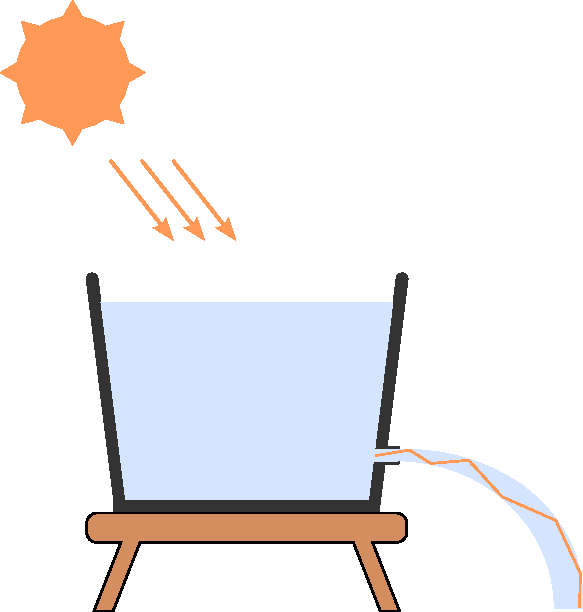
\includegraphics[width=0.45\textwidth]{lesson7/7-1_tyndall.pdf}
    \caption[Tyndall's experiment]{An early observation of light being guided by water pouring out of a bucket.}
    \label{fig:7-1_tyndall}
\end{figure}

One of the earliest demonstrations of guiding light in a waveguide was in an experiment by John Tyndall in 1870.
He filled a large vessel with water and let the water pour out from one of the sides.
He observed that light entering the water vessel did not exit the bucket through the hole in a straight line.
Remarkably, the light rays were guided by the water and seemingly followed the water's path.
Tyndall noticed that the rays were being reflected at the boundary between the water and air, confining them to stay within the streaming water.

This observation made many researchers investigate fiber optics and how to guide light, particularly in glass.
But it was only in 1960 with the invention of the laser when people truly realized the potential of using laser light coupled to fiber optics.
They spent a lot of effort in researching how to do that, and in 1966 people managed to couple lasers with fiber optics.
This really sparked the first information revolution (and was rewarded with a Nobel Prize in Physics for it).
Just to give you some idea how far we've come, in 1970 it was possible to transmit about one percent of the original light over a distance of one kilometer.
If you put in light of some power at the beginning, after one kilometer, you only had one hundredth of the original signal remaining.
Twenty years later, in 1990, it was possible to transmit 96\% of the original power over the same distance of one kilometer.

Let's have a quick look at what we're going to discuss in this chapter.
First, we're going to begin with two basic phenomena of how light behaves when it hits the interface of two materials.
We're going to talk about reflection and refraction.
These two are crucial for understanding how fiber optics works.
Then we will talk about total internal reflection where we're going to combine reflection and refraction and derive the condition for total internal reflection.
Total internal reflection is what we have seen in Tyndall's experiment, where light was not escaping the water stream but it was being reflected.
We will conclude by some basics of fiber optic cables, in particular how they are constructed and what the differences between various types of optical fibers are.


\section{Light at an interface}
\label{sec:7-2_light_at_interface}

In this section, we will look how light behaves when it travels from one medium to another.
To make this quantitative, we need a way to describe light. 
There are three major descriptions we can use, all useful in different circumstances.
Light can be viewed as a particle traveling in straight lines.
This scenario is described by \textit{\textbf{geometric optics}} and all that is required is some basic knowledge of trigonometry, making this scenario the easiest of the three to work with.

However, light possesses wave properties as well.
We have seen this on the example of the double-slit experiment in Section~\ref{sec:6-4_interference_single_photons}. 
In order to correctly account for these phenomena, we have to abandon geometric optics and resort to the use of \textit{\textbf{wave optics}}.
This description is necessary in some cases when light is travelling down a very narrow fiber.
In such a case we need the full power of Electromagnetism and Maxwell's equations.
This description is a lot harder and we're not going to use it here~\footnote{Maxwell's equations are covered in the second module in this series, "From Classical to Quantum Light".  They use partial differential equations (PDEs), which we briefly introduce in that module, but we recommend taking a math class that covers PDEs if you can. The more you have worked with PDEs the easier Maxwell's equations will be.}.

Finally, the third description is \textit{\textbf{quantum electrodynamics}}, because light is fundamentally a quantum field.
In this course, we will only use geometric optics.
There are a number of reasons for this.
Quantum electrodynamics describes interaction of light with matter at the atomic level.
We will not worry about such detailed description in this Chapter.
Similarly, wave optics are really only necessary for single-mode fibers that have cross-section $d$ comparable to the wavelength of light $\lambda$, where wave effects become important.
We will mainly discuss multi-mode fibers with cross-sections much larger than the wavelength of light.
Such fibers have cross-sections anywhere between $d=10$ micrometers to $d=200$ micrometers.
And they often carry light of wavelength $\lambda=1550$ nanometers.

\begin{figure}[t]
    \centering
    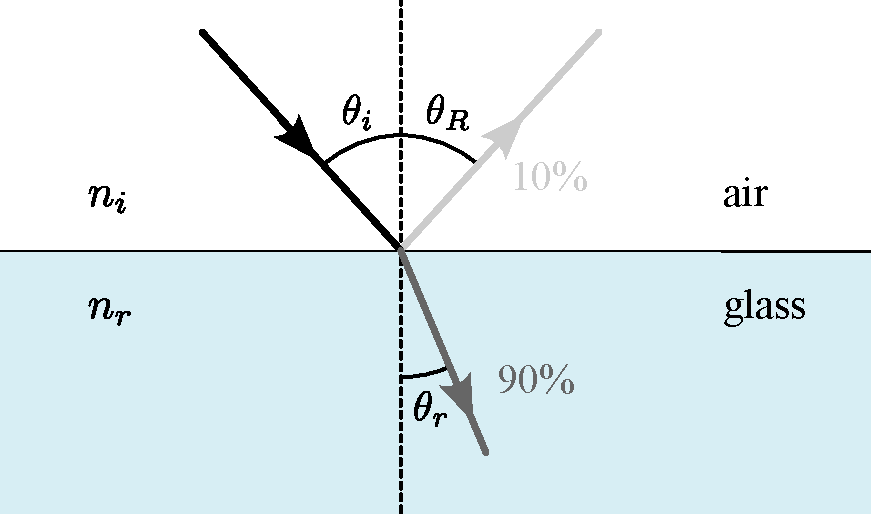
\includegraphics[width=0.65\textwidth]{lesson7/7-2_light-interface.pdf}
    \caption[Angle of incidence]{Light arriving at the interface between air and glass.}
    \label{fig:7-2_interface}
\end{figure}

Having settled on geometric optics as the means to describe how light behaves, let's see how to apply it to the case of light arriving at an interface of two different media.
To be more concrete, let's consider the light ray travelling in air, and being incident onto a piece of glass.
The \textit{\textbf{angle of incidence}} $\theta_i$ is measured with respect to the normal to the surface as shown in Fig.~\ref{fig:7-2_interface}.
At the interface between air and glass, portion of the incoming light is reflected back at the \textit{\textbf{angle of reflection}} $\theta_R$, again measured with respect to the normal.
The rest of the light enters the glass but the angle at which it travels changes to the \textit{\textbf{angle of refraction}} $\theta_r$.

The amount of light that is reflected and refracted is not important to our discussion right now, but we will return to it in our next module ``From Classical to Quantum Light''.
We are going to focus on the angles of reflection $\theta_R$ and refraction $\theta_r$.
The relationship between the angle of incidence and the angle of reflection is straightforward,
\begin{equation}
    \theta_R = \theta_i.
\end{equation}

The relationship between the angles of incidence and refraction is a little bit more involved.
We can observe from Fig.~\ref{fig:7-2_interface} that $\theta_r \neq \theta_i$.
Important quantity that helps with determining how much the angle of travel changes as light travels from one medium into another is the \textit{\textbf{refractive index}} $n$, defined as the ratio of the speed of light in vacuum $c$ and the speed of light in the medium $v$,
\begin{equation}
    n = \frac{c}{v}.
    \label{eq:7-2_refractive_index}
\end{equation}
Refractive index tells us how much the speed of light changes when travelling through different media.
The speed of light is greatest in vacuum and therefore $n\geq1$.
The refractive index of air is slightly larger than one, meaning that light slows down when travelling in air only very slightly.
Glass on the other hand, has a refractive index of $n_{glass} = 1.46$, meaning the light travels 1.46 times slower in the glass than when we compare it with the speed of light in vacuum.
Light slows down even more in diamond, which has refractive index of $n_{diamond} = 2.42$, giving diamond its unique and prized sparkling properties.

Let's return to the setting of Fig.~\ref{fig:7-2_interface}.
The light is initially travelling in some material, in our case air, at speed $v_i$, giving the refractive index $n_i = c / v_i$.
The refracted portion of light travels at a different speed $v_r$, resulting in refractive index $n_r = c / v_r$.
The angles of incident and refraction are related according to \textit{\textbf{Snell's law}},
\begin{equation}
    \frac{\sin\theta_i}{v_i} = \frac{\sin\theta_r}{v_r}.
\end{equation}
Using the relationship between the refractive index and the speed of light in a material in Eq.~(\ref{eq:7-2_refractive_index}), we can rewrite Snell's law in its more usual form,
\begin{equation}
    n_i \sin \theta_i = n_r \sin \theta_r.
    \label{eq:7-2_snell}
\end{equation}

\begin{figure}
    \centering
    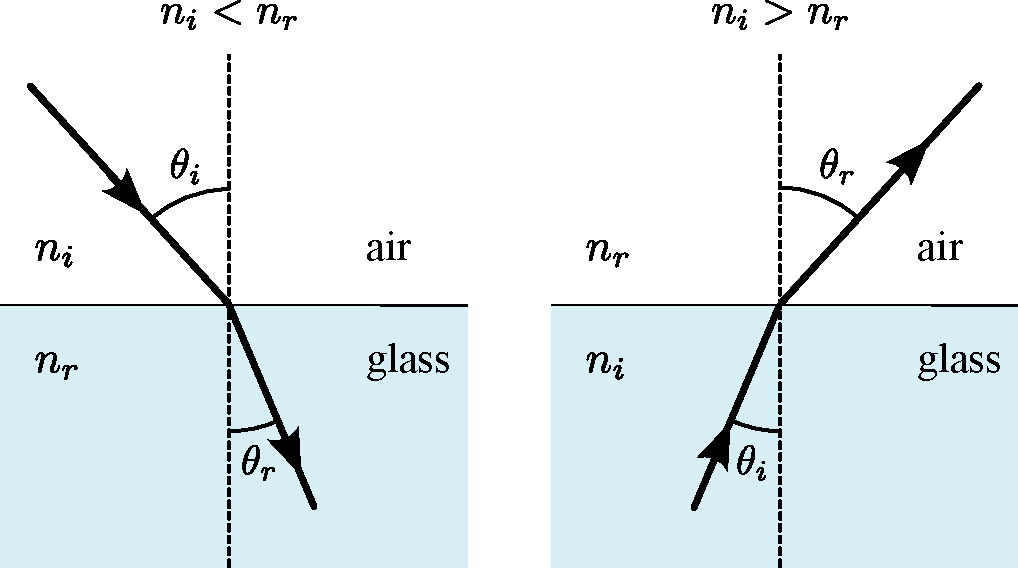
\includegraphics[width=0.7\textwidth]{lesson7/7-2_snell.pdf}
    \caption[Snell's law]{Angle of refraction can be larger or smaller than the angle of incidence.}
    \label{fig:7-2_snell_law}
\end{figure}

Using Snell's law of Eq.~(\ref{eq:7-2_snell}), let's look at how light behaves when entering into a new material.
We start with the case pictured on the left of Fig.~\ref{fig:7-2_snell_law}, where the light is travelling \textit{\textbf{from air to glass}}.
We can rearrange Eq.~(\ref{eq:7-2_snell}) to obtain
\begin{equation}
    \frac{n_i}{n_r} = \frac{\sin\theta_r}{\sin\theta_i}.
\end{equation}
Light travels faster in air than in glass, therefore we have $n_i / n_r < 1$.
This in turn means that $\sin\theta_r / \sin\theta_i < 1$ must be true.
This can be satisfied only when the angle of refraction is smaller than the angle of incidence,
\begin{equation}
    \theta_r < \theta_i, \qquad \text{when } \; n_i < n_r.
\end{equation}
We can also consider the opposite case when the light travels from \textit{\textbf{glass to air}}, as shown on the right of Fig.~\ref{fig:7-2_snell_law}.
This time, the refractive indices are reversed and we have $n_i > n_r$.
Repeating the same argument as above we discover that the light moves away from the normal to the surface,
\begin{equation}
    \theta_r > \theta_i, \qquad \text{when } \; n_i > n_r.
\end{equation}
This second case when light travels from a denser material to a less dense one will be studied in more detail in the next section.


\section{Total internal reflection}

\begin{figure}
    \centering
    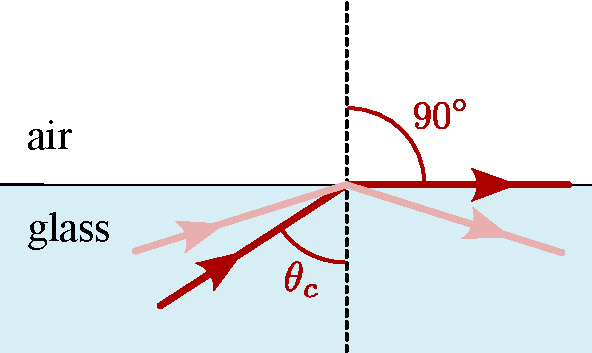
\includegraphics[width=0.4\textwidth]{lesson7/7-3_total_internal_reflection.pdf}
    \caption[Total internal reflection]{At the critical angle, light travels just along the surface of the glass.}
    \label{fig:7-3_total_internal_reflection}
\end{figure}
We saw that if light is incident on an interface between two materials and traveling from a more dense material into a less dense one, then it gets refracted away from the normal.
The angle of refraction is larger than the angle of incidence, $\theta_r > \theta_i$. Consider the scenario where we are steadily increasing the angle of incidence as pictured in Fig.~\ref{fig:7-3_total_internal_reflection}.
The refracted beam is moving correspondingly moving further away from the normal.
An interesting question to ask is at what angle of incidence will the refracted beam travel parallel to the surface between the two materials.
We can answer this question by setting $\theta_r=90^{\circ}$ in Eq.~(\ref{eq:7-2_snell}).
The \textit{\textbf{critical angle}} $\theta_c$ is the angle at which this is true, s owe also replace the angle of incidence $\theta_i$ with $\theta_c$,
\begin{equation}
    n_i \sin \theta_c = n_r \sin 90^{\circ}.
    \label{eq:7-4_crit_angle}
\end{equation}
Using $\sin 90^{\circ} = 1$, we can obtain an expression for the critical angle,
\begin{equation}
    \theta_c=\sin ^{-1}\left(\frac{n_r}{n_i}\right).
    \label{eq:7-3_crit_angle}
\end{equation}

%We have that the $n_i$, the refractive index of glass, times the sine of the angle of incidence, is equal to the refractive index of air $n_r$, times the sine of $\theta_r$, but we know that here we are looking for a scenario where the sine of $\theta_r$ is just sine of ninety degrees which is equal to one. So we have the following relationship (see pointer), and we have changed the subscript here on this $\theta$ to "$\theta_c$" which stands for "critical angle", because that's the critical angle where we obtain angle of refraction of ninety degrees. Now we can just rearrange to get sine of $\theta_c$, equal to as a simple fraction of $n_r / n_i$. In our case, here $n_r$ is the refractive index of air and $n_i$ is the refractive index of glass, and we can just take the arc sine ($\sin^{-1}$) to obtain this expression for the critical angle. 

When light is at this angle $\theta_c$, then after reaching the interface the light ray travels parallel to the surface.
We can keep increasing the angle of incidence so that $\theta_i > \theta_c$.
In this case, all of the light gets reflected back, undergoing \textit{\textbf{total internal reflection}}.
This is the basic working principle behind optical fibers and it is in fact responsible for observations made by Tyndall in his experiment.

\begin{figure}
    \centering
    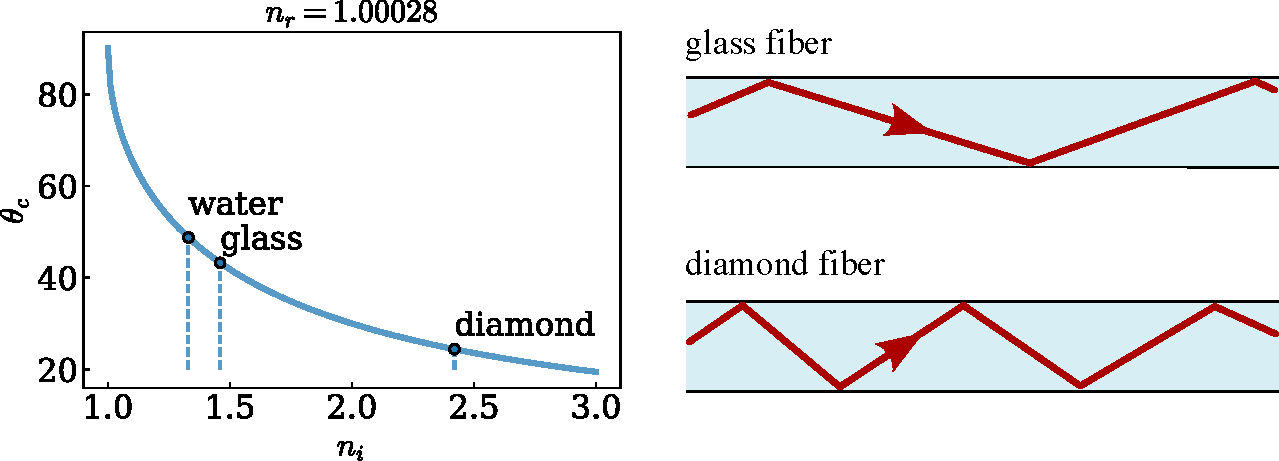
\includegraphics[width=0.9\textwidth]{lesson7/7-3_crit_angle.pdf}
    \caption[Critical angle]{Critical angle gets smaller as the refractive index increases.}
    \label{fig:7-3_crit_angle}
\end{figure}

In the left panel of Fig.~\ref{fig:7-3_crit_angle}, we can the plot of how the critical angle $\theta_c$ changes with the refractive index $n_i$ of the material the waveguide is made from.
We assume that the material outside of the waveguide is still just air with a refractive index of $n_r = 1.00028$.
As the refractive index of the waveguide increases, the critical angle decreases.
This has important implications for the design of an optical fiber.
Fibers with smaller refractive indices must ensure that the light is incident on the surface at a larger angle, otherwise the light will escape.
On the other hand, fibers made from material with high refractive index make very good waveguides because they are capable of containing the light better as shown in the right panel of Fig.~\ref{fig:7-3_crit_angle}.



\section{Optical fibers}
\label{sec:7-4_optical fibers}

\begin{figure}[t]
    \centering
    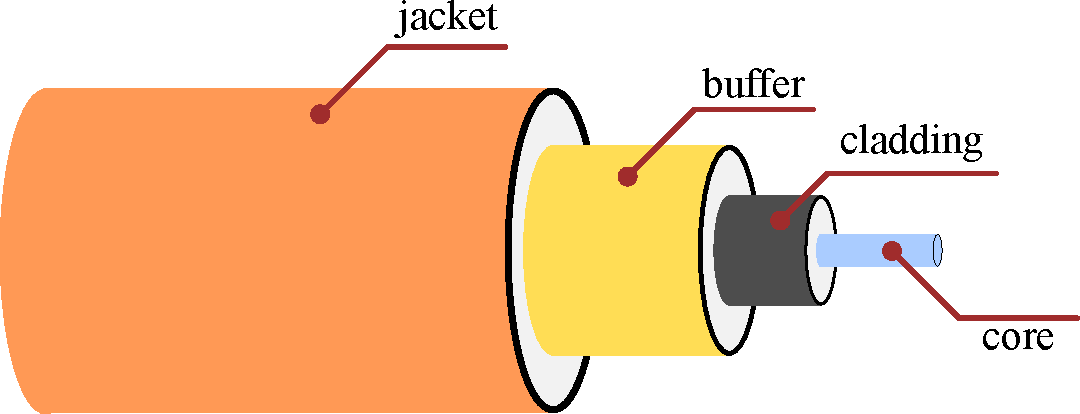
\includegraphics[width=0.7\textwidth]{lesson7/7-4_fiber.pdf}
    \caption[Anatomy of an optical fiber]{Anatomy of an optical fiber.}
    \label{fig:7-4_fiber}
\end{figure}

Let's have a look at the composition of a typical optical fiber\index{optical fiber}.
Often, many fibers are bundled into a fiber-optic cable, but here we will look at an individual fiber as shown in Fig.~\ref{fig:7-4_fiber}. 
The outermost layer is the \textit{\textbf{jacket}}.
Its function is to protect the inside components of the fiber from the environment.
Under the jacket is the \textit{\textbf{buffer}}.
The buffer offers further protection, and sometimes bundles multiple optical fibers.
The next layer under the buffer is the \textit{\textbf{cladding}}.
This is the material that is responsible for reflecting light back and keeping it contained within the innermost layer, which is the \textit{\textbf{core}}.
Cladding serves as a form of protection and prevents cross-talk in the case of multiple fibers bundled within the buffer.
Having two cores next to each other would result in light leaking from one core to the other.
The refractive index of the cladding must be smaller than the refractive index of the core in order for the light signal to have a chance of undergoing total internal reflection.

\begin{figure}[t]
    \centering
    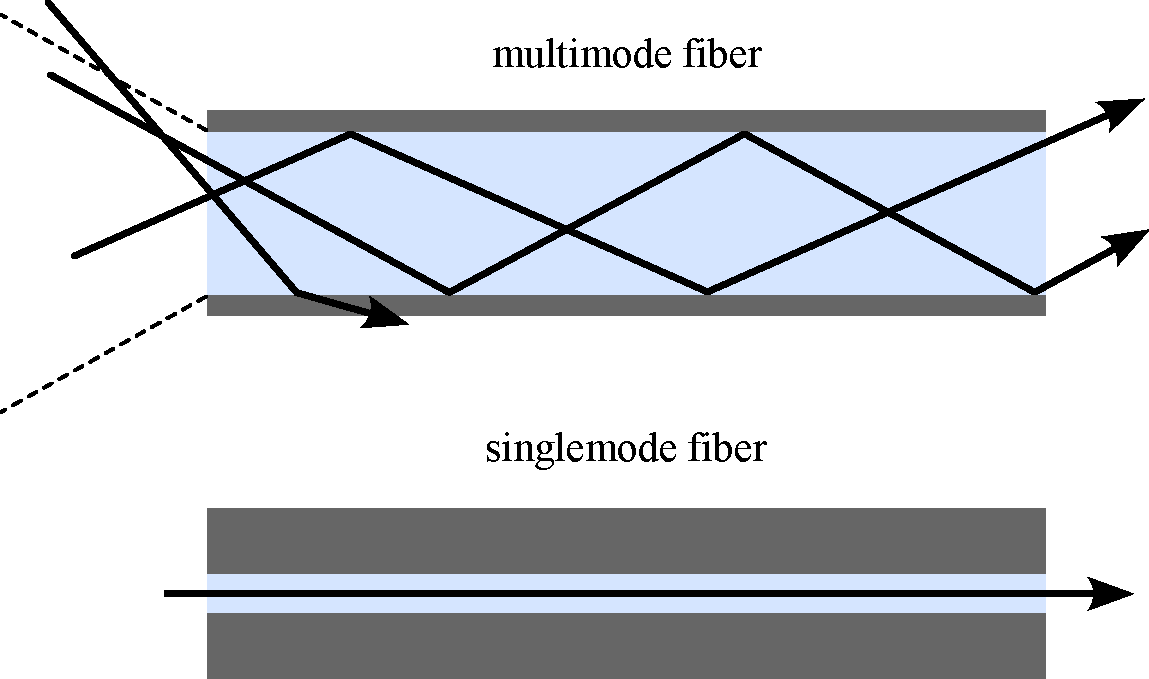
\includegraphics[width=0.7\textwidth]{lesson7/7-4_multi_single_fiber.pdf}
    \caption[Multimode and singlemode fibers]{Two main types of optical fibers, multimode and singlemode.}
    \label{fig:7-4_multimode_singlemode_fiber}
\end{figure}

Depending on the thickness of the core, optical fibers are classified into two types as shown in Fig.~\ref{fig:7-4_multimode_singlemode_fiber}.
\textit{\textbf{Multimode fiber}}\index{multimode fiber} has cross-section diameter much larger than the wavelength of light.
The mode of light here refers to the spatial direction in which each beam of light travels.
The multimode fiber in Fig.~\ref{fig:7-4_multimode_singlemode_fiber} has three modes coupling to it but only two modes making the journey all the way to the end.
We will discuss why this is shortly.
\textit{\textbf{Singlemode fiber}} \index{single-mode fiber} has cross-section diameter comparable with the wavelength of light and is able to support only a single mode of light.
This mode is called \textit{\textbf{transverse mode}} \index{transverse mode} of light.

Let's look at multimode fibers first.
Figure~\ref{fig:7-4_multimode_singlemode_fiber} shows one of the modes of light being lost in the multimode fiber.
This mode leaks out of the fiber due to its angle of incidence onto the cladding being less than the critical angle.
Modes of light can couple to a multimode fiber only if they are within the \textit{\textbf{acceptance cone}} \index{acceptance angle}, represented by the dashed lines.
Any modes that arriving at the entrance of the fiber from outside of this cone will be refracted by the cladding and leak out of the fiber.
This suggests there is a relationship between the angle of acceptance and the critical angle.

\begin{figure}[t]
    \centering
    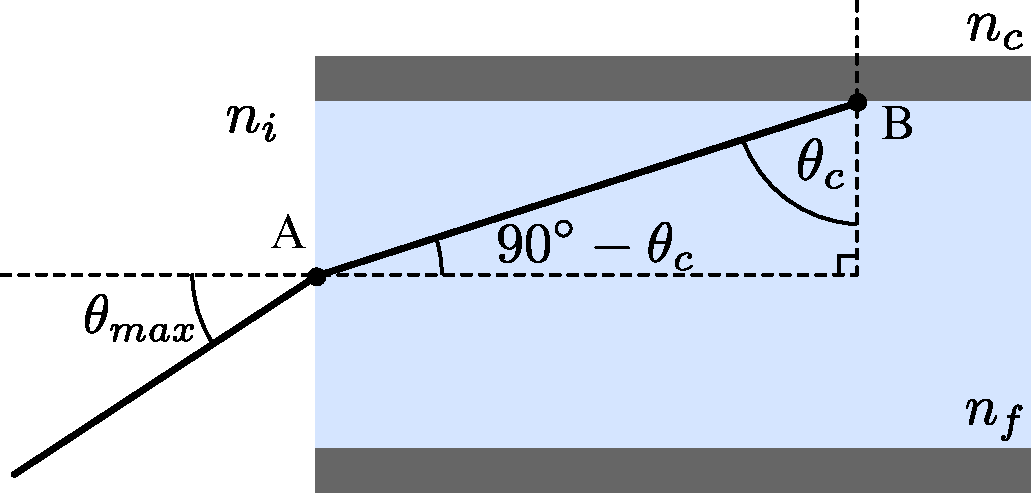
\includegraphics[width=0.6\textwidth]{lesson7/7-4_acceptance_cone.pdf}
    \caption[Acceptance cone]{Maximum incidence angle of the light beam onto the fiber's core such that it hits the cladding at the critical angle.}
    \label{fig:7-4_acceptance_cone}
\end{figure}

Let's make this relationship more quantitative.
Consider the situation of Fig.~\ref{fig:7-4_acceptance_cone} where a light beam is incident onto the core of a fiber at point $A$, gets refracted, and is later incident onto the cladding at point $B$.
Our aim is to find the maximum angle of incidence $\theta_{max}$ onto the core such that angle of incidence onto the cladding is the critical angle $\theta_c$.
We denote the refractive index of the material outside the fiber by $n_i$, the refractive index of the core by $n_f$, and the refractive index of the cladding by $n_c$.
Using Snell's law at point $A$, we have $n_i \sin \theta_i = n_f \sin \theta_r$.
We can use the right-hand triangle in Fig.~\ref{fig:7-4_acceptance_cone} to see that $\theta_r = 90^{\circ} - \theta_c$.
In that case we can set the incidence angle at point $A$ to $\theta_i = \theta_{max}$,
\begin{equation}
    n_i \sin \theta_{max} = n_f \sin (90^{\circ} - \theta_c).
\end{equation}
Using the trigonometric identity $\sin(\theta + \phi) = \sin\theta\cos\phi + \sin\phi\cos\theta$, we obtain
\begin{equation}
    n_i \sin \theta_{max} = n_f \cos\theta_c,
\end{equation}
where we used $\cos(-\theta_c) = \cos\theta_c$.
We express the cosine of the the critical angle in terms of sine, $\cos\theta_c = \sqrt{1 - \sin^2\theta_c}$, and using Eq.~(\ref{eq:7-3_crit_angle}),
\begin{equation}
    n_i \sin \theta_{max} = n_f \sqrt{1 - \left( \frac{n_c}{n_f} \right)^2}.
\end{equation}
Bringing the refractive index of the fiber under square root, we obtain
\begin{equation}
    n_i \sin \theta_{max} = \sqrt{n_f^2 -  n_c^2}.
    \label{eq:7-4_theta_max}
\end{equation}
The expression on the left of Eq.~(\ref{eq:7-4_theta_max}), $n_i \sin \theta_{max}$, is known as \textit{\textbf{numerical aperture}} \index{numerical aperture}.
Larger numerical aperture means that it is easier to couple to the fiber as the acceptance cone is wider.
Equation~(\ref{eq:7-4_theta_max}) allows us to calculate the maximum incidence angle given the three refractive indices $n_i$, $n_c$, and $n_f$.
The acceptance cone is given by twice this angle, $2 \theta_{max}$.

We said that the diameter of the core for a multimode fiber is much larger than the wavelength of light, leading to core being able to support a number of modes.
The speed of light in the core is the same for all these modes, however the time it takes for individual modes to reach the end of the fiber is different.
Due to the different angles of incidence of different modes, they have to cover different total distances before reaching the end.
This is known as \textit{\textbf{mode dispersion}} \index{mode dispersion}.
We will cover mode dispersion in more detail in Section~\ref{sec:11-2_mode_dispersion}.
Because of this, multimode fibers are more suitable for short distances, such as in office and campus networks.
On the other hand, because the core does not need to extremely small, multimode fibers are easier to manufacture leading to savings in production costs.

In contrast, singlemode fibers are much more difficult to produce, as their core diameter is typically less than $10$ micrometers.
For comparison, the average width of a human hair is larger than $20$ micrometers.
Singlemode fibers support only the transverse mode, therefore there is no mode dispersion.
Mode dispersion changes the shape of the signal received at the far end, so the rate at which a signal can be changed while maintaining a clean signal at the receiver is determined by the amount of this dispersion.
Singlemode fibers allow for high rate of transfer of data, making them suitable for long distance communications.
They have to be boosted by repeaters approximately every 50 kilometers because they are still susceptible to attenuation.
We will discuss how to combat attenuation in Section~\ref{sec:11-4_overcoming_losses}.

\begin{figure}[t]
    \centering
    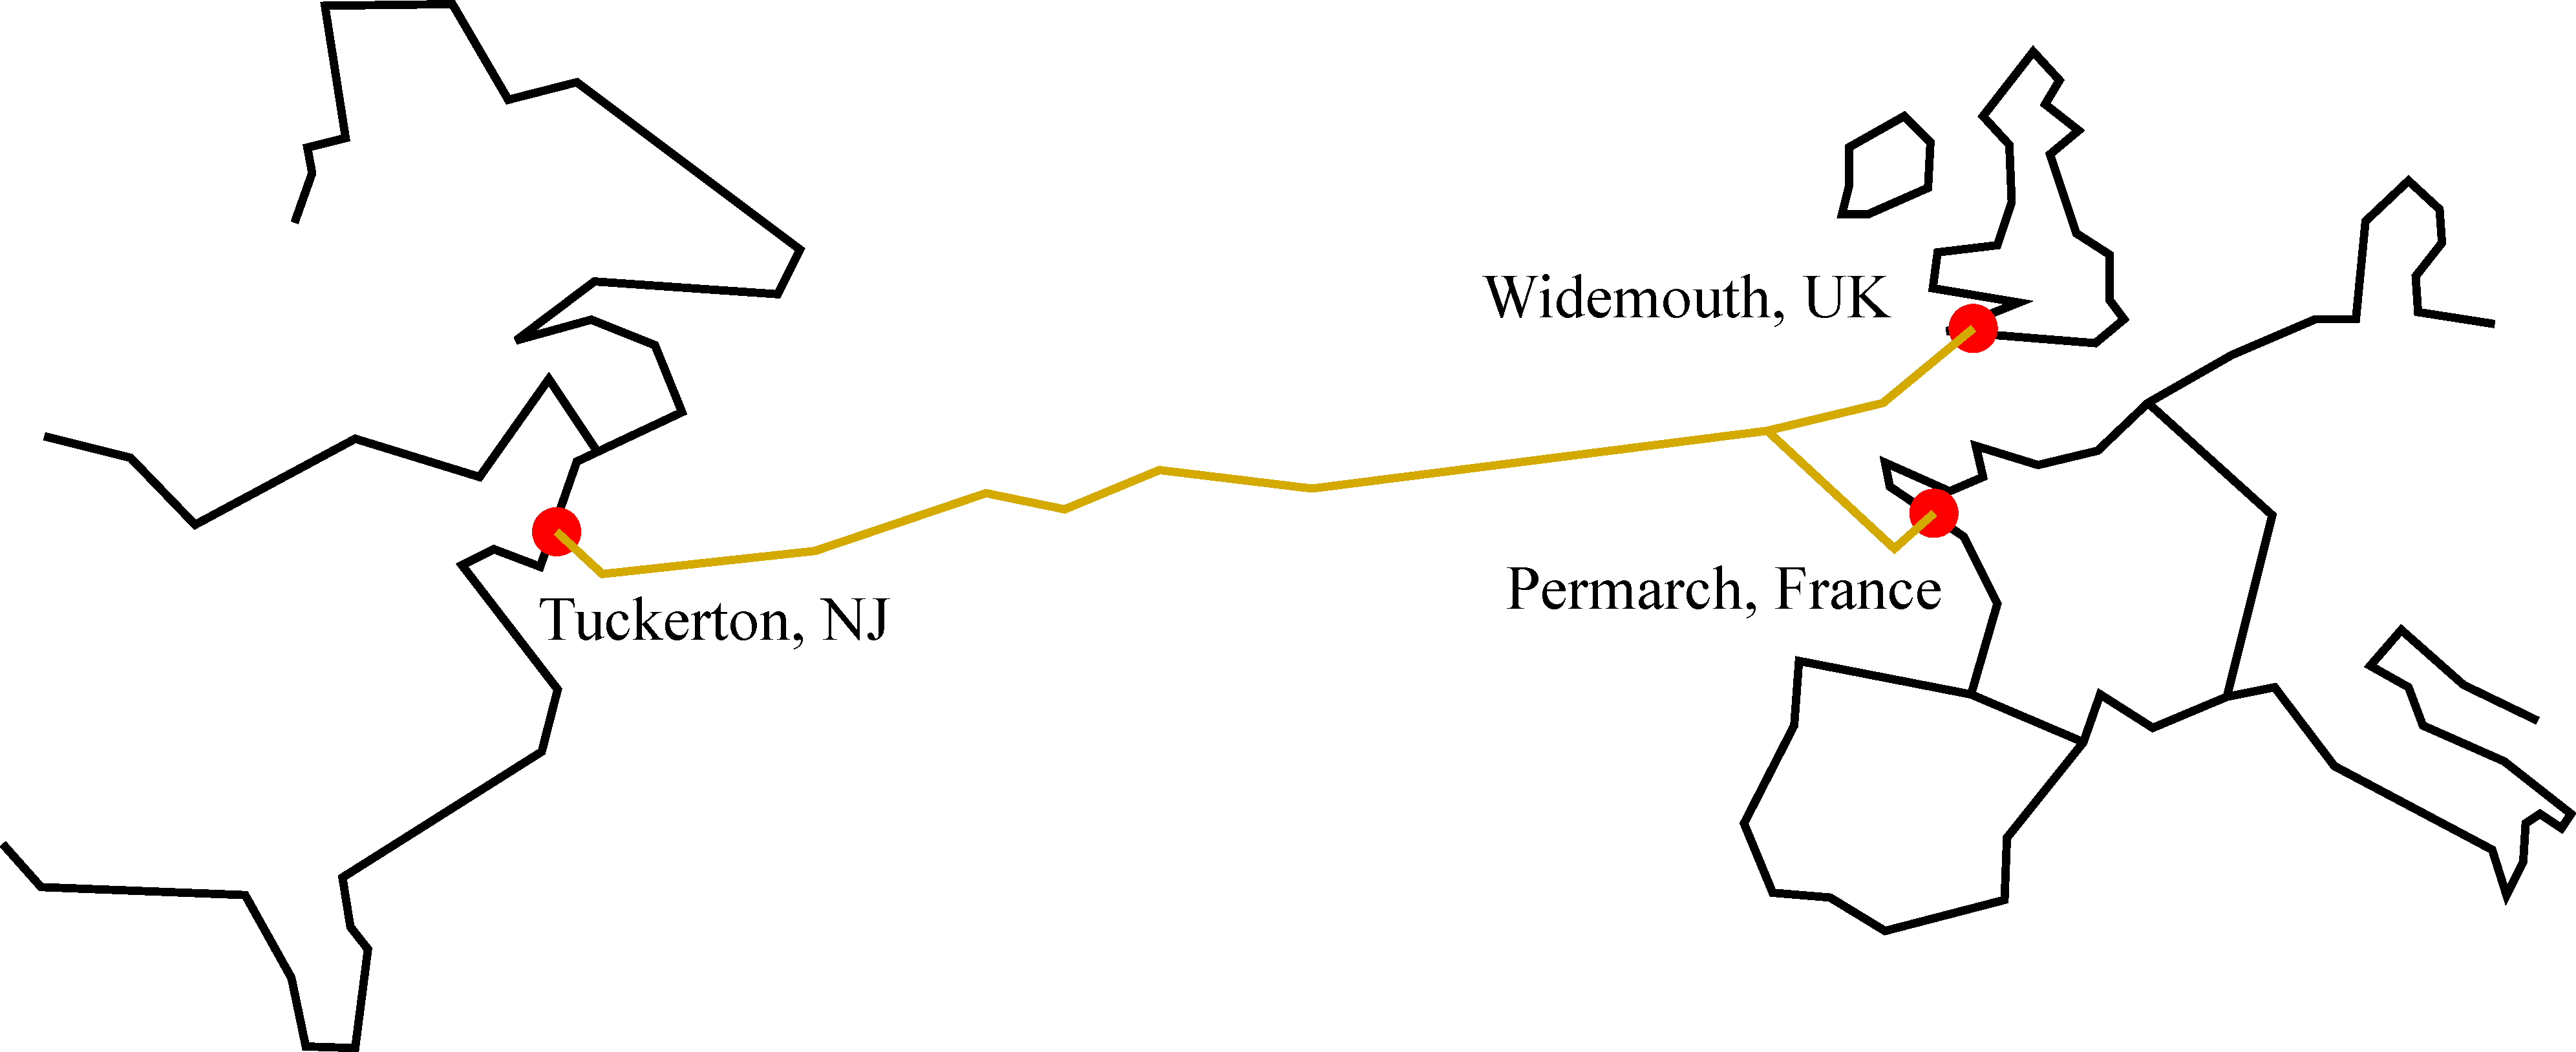
\includegraphics[width=\textwidth]{lesson7/7-4_TAT8.pdf}
    \caption[TAT-8]{The first transatlantic communications cable, TAT-8.}
    \label{fig:7-4_TAT8}
\end{figure}

The first transatlantic fiber optic cable, called TAT-8, was laid in 1988 between Tuckerton, New Jersey, and the UK and France.
The submarine cable was constructed at a cost of approximately 335 million US dollars, and it was retired in 2002.
It was predicted that the bandwidth of this fiber optic cable would last for a long time and probably will never be reached.
The bandwidth was 280 Mbits/s, which can carry around 40,000 phone circuits simultaneously.
This capacity was reached in eighteen months, necessitating the laying of more cables.

\newpage
\begin{exercises}
\exer{Consider the following quantum state:}
\begin{equation*}
\ket{\psi} = \frac{\sqrt{3}}{2}\ket{0} + \frac{1}{2}\ket{1}
\end{equation*}
\subexer{Find the probability of measuring a zero.}
\subexer{Find the probability of measuring a one.}


\end{exercises}

\newpage
\section*{Quiz}
  \addcontentsline{toc}{section}{Quiz}

\section*{Further reading Chapters 5-7}
  \addcontentsline{toc}{section}{Further reading Chapters 5-7}

Chapter 5

This Chapter discusses the various types of light depending on their coherence properties. Coherent light produced by lasers is crucially important from the perspective of communication. A good qualitative as well as quantitative introduction to lasers can be found in Chapter 1 of:

Orazio Svelto, Principles of Lasers, Springer, 2009.

A great discussion of lasing behaviour from the perspective of a mathematician (but still explained very intuitively) is in Chapter 3 of the classic:

Steven H. Strogatz, Nonlinear Dynamics and Chaos: With Applications to Physics, Biology, Chemistry, and Engineering, CRC Press, 2000.

Chapter 6

Two great optics textbooks for this Block as well as the following ones are:

Eugene Hecht, Optics, Pearson, 2015.
Grant R. Fowles, Introduction to Modern Optics, Dover Publications, 1989.

Bahaa E. A. Saleh, Malvin C. Twitch, Fundamentals of Photonics, Wiley-Interscience, 2007.

These books focus on wave and geometric optics and provide a good foundation for transitioning to quantum optics which we will do later. The former is a common undergraduate textbook, while the latter is more advanced and contains a lot of specialized information, perhaps best suited to those planning further study in optics.

Interference is an extremely important concept. We encourage you to read and understand the discussion in Chapter 1 in:

Richard P. Feynman, Robert P. Leighton, Matthew Sands, The Feynman Lectures on Physics, Vol. 3, Addison Wesley, 1971.

Chapter 7

This Chapter relies mainly on the geometric description of light propagation. Section 4.3 and Section 5.6 of Hecht’s textbook contain great discussion of reflection and propagation in optical fibers, respectively.
